 \documentclass[12pt]{article}
\setlength\parindent{0pt}
\usepackage{amsmath}
\usepackage{lscape}
\usepackage{graphicx}
\usepackage{fullpage}
\usepackage[margin=0.8in]{geometry}
\setlength{\parskip}{4mm}
\def\LL{\left\langle}   % left angle bracket
\def\RR{\right\rangle}  % right angle bracket
\def\LP{\left(}         % left parenthesis
\def\RP{\right)}        % right parenthesis
\def\LB{\left\{}        % left curly bracket
\def\RB{\right\}}       % right curly bracket
\def\PAR#1#2{ {{\partial #1}\over{\partial #2}} }
\def\PARTWO#1#2{ {{\partial^2 #1}\over{\partial #2}^2} }
\def\PARTWOMIX#1#2#3{ {{\partial^2 #1}\over{\partial #2 \partial #3}} }
\newcommand{\BE}{\begin{displaymath}}
\newcommand{\EE}{\end{displaymath}}
\newcommand{\BNE}{\begin{equation}}
\newcommand{\ENE}{\end{equation}}
\newcommand{\BEA}{\begin{eqnarray}}
\newcommand{\EEA}{\nonumber\end{eqnarray}}
\newcommand{\EL}{\nonumber\\}
\newcommand{\la}[1]{\label{#1}}
\newcommand{\ie}{{\em i.e.\ }}
\newcommand{\eg}{{\em e.\,g.\ }}
\newcommand{\cf}{cf.\ }
\newcommand{\etc}{etc.\ }
\newcommand{\Tr}{{\rm tr}}
\newcommand{\etal}{{\it et al.}}
\newcommand{\OL}[1]{\overline{#1}\ } % overline
\newcommand{\OLL}[1]{\overline{\overline{#1}}\ } % double overline
\newcommand{\OON}{\frac{1}{N}} % "one over N"
\newcommand{\OOX}[1]{\frac{1}{#1}} % "one over X"
\pagenumbering{gobble}

\begin{document}
\Large
\centerline{\sc{Quiz 2 -- The Motion of the Zodiac}}

\begin{minipage}{0.6\textwidth}
	\Large
	Name: \underline{\hspace{3in}}
\end{minipage}
\begin{minipage}{0.4\textwidth}
	\Large
	Lab Section: M0\underline{\hspace{1in}}\\
	\small (if you want your paper back)
\end{minipage}

\normalsize

For this quiz, you may use your Homework 2 or anything you yourself have handwritten, but may not consult with anyone else or use electronic devices.

Turn your paper into the boxes by the doors.



\begin{center}
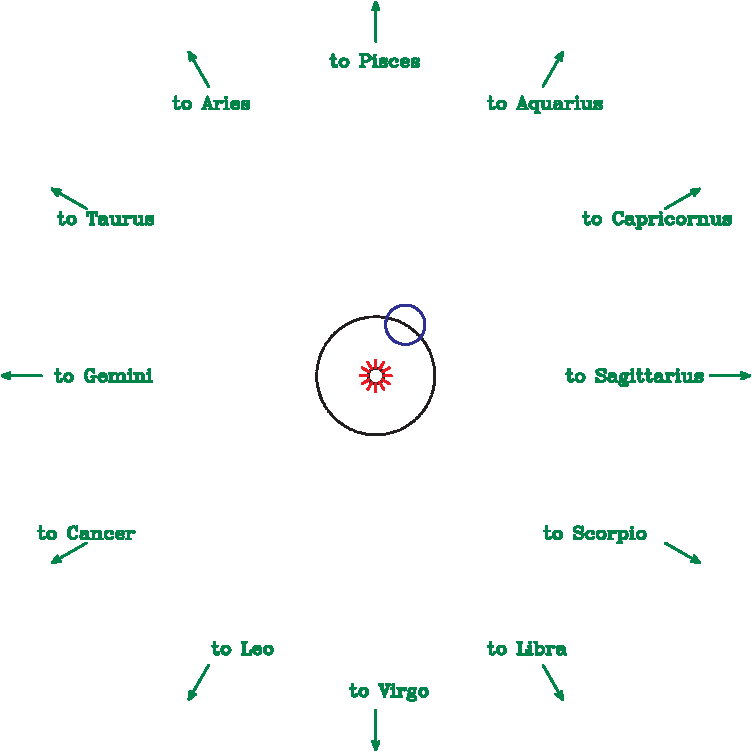
\includegraphics[width=6in]{earth-orbit-quiz-crop.pdf}

\it This is a diagram of the Earth in September, seen from above the North Pole. From this perspective, the Earth rotates on its axis counterclockwise and orbits the Sun counterclockwise.

\bigskip

The questions are on the back page.

\end{center}
\newpage


\begin{enumerate}
	\item Draw a stick figure in a location on the Earth (shown in the diagram) that is shortly after sunset.
	
	\item Which constellations in the Zodiac would your observer see:
	
	\begin{enumerate}
		\item Low above the eastern horizon
		\vspace{0.5in}
		
		\item High in the sky
				\vspace{0.5in}
		\item Low above the western horizon
				\vspace{0.5in}
	\end{enumerate}

\item How long would your observer need to wait after September before the constellation Virgo was directly behind the Sun? {\it (The Earth drawn on the diagram is in September.)}

\vspace{1in}

\item Four months after September, an observer looks up at the sky at midnight. What constellations in the Zodiac would they see:

\begin{enumerate}
	\item Low above the eastern horizon		\vspace{0.5in}
	\item High in the sky		\vspace{0.5in}
	\item Low above the western horizon
\end{enumerate}

	
	


\end{enumerate}





\end{document}

